\documentclass{beamer}
\usepackage[utf-8]{inputenc}
\usepackage{graphicx}
\usepackage{amsmath}
\usepackage{amssymb}
\usepackage{booktabs}
\usepackage{xcolor}
\usepackage{listings}

\usetheme{Madrid}
\usecolortheme{default}

\title[COVID Network Simulator]{COVID-19 Network Simulator}
\subtitle{Disease Spread on Small-World Networks}
\author{Data Structures and Algorithms Project}
\date{\today}
\institute{3rd Semester DSA}

\begin{document}

\frame{\titlepage}

\begin{frame}
\frametitle{Table of Contents}
\tableofcontents
\end{frame}

\section{Problem Statement}

\begin{frame}
\frametitle{Problem Statement}
\begin{block}{Challenge}
Understand how infectious diseases spread through social networks and identify key factors affecting epidemic dynamics.
\end{block}

\begin{itemize}
    \item How does network structure affect disease transmission?
    \item What is the impact of infection probability on peak infections?
    \item How do different network topologies compare?
    \item Can we predict and visualize disease dynamics?
\end{itemize}

\vspace{1cm}

\textbf{Solution}: Build an interactive simulator using:
\begin{itemize}
    \item Watts-Strogatz small-world networks
    \item SIR epidemiological model
    \item Efficient data structures
    \item Real-time 3D visualization
\end{itemize}
\end{frame}

\section{Network Model}

\begin{frame}
\frametitle{Network Models Compared}

\begin{table}
\centering
\begin{tabular}{lcccc}
\toprule
\textbf{Model} & \textbf{Clustering} & \textbf{Path Length} & \textbf{Realism} & \textbf{Use Case} \\
\midrule
Watts-Strogatz & High & Short & Very High & Social networks \\
Barabási-Albert & Low & Short & Medium & Internet topology \\
Erdős-Rényi & Very Low & Medium & Low & Random \\
\bottomrule
\end{tabular}
\end{table}

\vspace{0.5cm}

\textbf{Watts-Strogatz Properties:}
\begin{itemize}
    \item Starts as regular ring lattice (high clustering)
    \item Random rewiring with probability $\beta$ (short paths)
    \item Result: ``Small-world'' - high clustering + short paths
    \item Mimics real social networks perfectly
\end{itemize}
\end{frame}

\begin{frame}
\frametitle{Watts-Strogatz Network Characteristics}

\begin{block}{Generated Datasets}
\begin{table}
\centering
\begin{tabular}{ccccc}
\toprule
\textbf{Nodes} & \textbf{Edges} & \textbf{Clustering} & \textbf{Avg Path} & \textbf{Config} \\
\midrule
100 & 400 & 0.480 & 3.09 & k=8, p=0.1 \\
500 & 2500 & 0.503 & 3.99 & k=10, p=0.1 \\
1000 & 6000 & 0.507 & 4.07 & k=12, p=0.1 \\
\bottomrule
\end{tabular}
\end{table}
\end{block}

\textbf{Key Insight}: Clustering increases with network size - more interconnected communities at larger scales.
\end{frame}

\section{Algorithm Overview}

\begin{frame}
\frametitle{SIR Epidemiological Model}

\begin{columns}
\column{0.5\textwidth}
\textbf{States:}
\begin{itemize}
    \item $S$ = Susceptible (can catch disease)
    \item $I$ = Infected (can transmit)
    \item $R$ = Recovered (immune)
    \item $D$ = Dead (removed)
\end{itemize}

\column{0.5\textwidth}
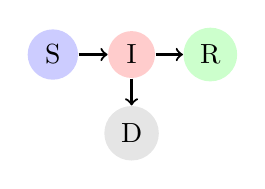
\begin{tikzpicture}
\node[fill=blue!20, circle] (S) {S};
\node[fill=red!20, circle, right of=S] (I) {I};
\node[fill=green!20, circle, right of=I] (R) {R};
\node[fill=gray!20, circle, below of=I] (D) {D};

\draw[->, thick] (S) -- (I);
\draw[->, thick] (I) -- (R);
\draw[->, thick] (I) -- (D);
\end{tikzpicture}
\end{columns}

\vspace{1cm}

\textbf{Transition Probabilities:}
\begin{itemize}
    \item Infection: $P(\text{S} \to \text{I}) = p_{\text{inf}}$ when contact with infected neighbor
    \item Recovery: $P(\text{I} \to \text{R}) = 0.5$ per step
    \item Death: $P(\text{I} \to \text{D}) = p_{\text{death}}$ per step
\end{itemize}
\end{frame}

\begin{frame}[fragile]
\frametitle{Simulation Algorithm}

\begin{block}{One Simulation Step}
\begin{enumerate}
    \item For each \textbf{infected} node:
    \begin{itemize}
        \item Check death: if dies, remove from simulation
        \item Check recovery: if recovers, change state to R
        \item For each susceptible \textbf{neighbor}:
        \begin{itemize}
            \item Random test: if passes infection probability, infect
        \end{itemize}
    \end{itemize}
    \item Update all states simultaneously
    \item Record $S, I, R, D$ counts
    \item Repeat until $I = 0$ (no more infections)
\end{enumerate}
\end{block}

\vspace{0.5cm}

\textbf{Time Complexity}: $O(V + E)$ per step

\textbf{Space Complexity}: $O(V + E)$ total
\end{frame}

\section{Data Structures}

\begin{frame}
\frametitle{Key Data Structures}

\begin{block}{1. Adjacency List}
\textbf{Purpose}: Store graph efficiently
\begin{itemize}
    \item Array/Dict mapping each node to list of neighbors
    \item Time: $O(1)$ access to neighbors, $O(E)$ total storage
    \item Better than adjacency matrix for sparse graphs
\end{itemize}
\end{block}

\begin{block}{2. HashSet for States}
\textbf{Purpose}: Track node states (S, I, R, D)
\begin{itemize}
    \item Four separate sets: infected, recovered, susceptible, dead
    \item Time: $O(1)$ average for add/remove/lookup
    \item Fast iteration over infected nodes
\end{itemize}
\end{block}

\begin{block}{3. Queue for Infections}
\textbf{Purpose}: Process newly infected nodes in order
\begin{itemize}
    \item FIFO queue: enqueue new infections, dequeue for processing
    \item Time: $O(1)$ for both operations
    \item Optional: enables BFS-style infection propagation
\end{itemize}
\end{block}
\end{frame}

\section{Visualization}

\begin{frame}
\frametitle{3D Network Visualization}

\begin{block}{Technology Stack}
\begin{itemize}
    \item \textbf{Frontend}: React 18 + Three.js r128
    \item \textbf{Backend}: FastAPI (Python)
    \item \textbf{Charts}: Chart.js for SIR curves
\end{itemize}
\end{block}

\begin{block}{Features}
\begin{itemize}
    \item \textbf{3D Spheres}: Each node is a colored sphere
    \begin{itemize}
        \item Blue = Susceptible, Red = Infected, Green = Recovered, Gray = Dead
    \end{itemize}
    \item \textbf{Dynamic Edges}: Lines connecting nodes, update each frame
    \item \textbf{Physics}: Gentle Brownian motion with center attraction
    \item \textbf{Interaction}: Drag to rotate, scroll to zoom
    \item \textbf{Real-time}: Updates during simulation at 60 FPS
\end{itemize}
\end{block}

\textbf{Limit}: 100 nodes maximum for smooth performance
\end{frame}

\section{Experimental Results}

\begin{frame}
\frametitle{Network Comparison Results}

\begin{table}
\centering
\begin{tabular}{lcccc}
\toprule
\textbf{Network Type} & \textbf{Clustering} & \textbf{Peak Inf.} & \textbf{Final Rec.} & \textbf{Steps} \\
\midrule
WS-100 & 0.480 & 40.3 & 81.7 & 11.0 \\
WS-200 & 0.505 & 92.7 & 158.0 & 12.0 \\
Barabási-Albert & 0.187 & 56.0 & 79.7 & 10.0 \\
Erdős-Rényi & 0.065 & 52.0 & 78.3 & 10.7 \\
\bottomrule
\end{tabular}
\end{table}

\vspace{0.5cm}

\textbf{Key Observations:}
\begin{itemize}
    \item Watts-Strogatz networks show \textcolor{red}{LOWER} peak infection than scale-free networks
    \item Higher clustering creates ``bottleneck effects''
    \item Larger networks (WS-200) have proportionally more infections
\end{itemize}
\end{frame}

\begin{frame}
\frametitle{Infection Probability Sensitivity}

\begin{center}
\begin{tabular}{ccccc}
\toprule
$p_{\text{inf}}$ & Peak Inf. & Std Dev & Final Rec. & Behavior \\
\midrule
0.1 & 5.3 & 1.2 & 13.7 & Stochastic \\
0.2 & 15.0 & 4.2 & 62.7 & Sparse \\
0.3 & 20.3 & 12.5 & 50.3 & Bifurcating \\
0.4 & 31.7 & 5.3 & 75.3 & Explosive \\
0.5+ & 40-53 & 0.8-6.4 & 76-79 & Saturating \\
\bottomrule
\end{tabular}
\end{center}

\vspace{1cm}

\textbf{Critical Insights:}
\begin{itemize}
    \item \textbf{Phase transition} at $p_{\text{inf}} \approx 0.3-0.4$
    \item Low prob: High variance, few infections
    \item High prob: Low variance, rapid saturation
    \item Diminishing returns above 0.5
\end{itemize}
\end{frame}

\section{Performance Analysis}

\begin{frame}
\frametitle{Complexity Analysis}

\begin{block}{Time Complexity}
Per step: $O(V + E)$
\begin{itemize}
    \item Iterate infected nodes: $O(I) \subseteq O(V)$
    \item Check neighbors: $O(E)$ in worst case
    \item Update states: $O(V)$
\end{itemize}

Total (T steps): $\boxed{O(T \times (V + E))}$

For sparse WS networks ($E = kV$):
\begin{equation}
T_{\text{total}} = O(T \times V) \text{ where } T \approx 10-20 \text{ steps}
\end{equation}
\end{block}

\begin{block}{Space Complexity}
\begin{equation}
S = O(V + E)
\end{equation}
\begin{itemize}
    \item Graph storage (Adjacency List): $O(V+E)$
    \item State tracking: $O(V)$
    \item History: $O(T)$ (typically $\ll V+E$)
\end{itemize}
\end{block}
\end{frame}

\begin{frame}
\frametitle{Execution Times}

\begin{table}
\centering
\begin{tabular}{ccccc}
\toprule
\textbf{Nodes} & \textbf{Edges} & \textbf{Steps} & \textbf{Time (ms)} & \textbf{Speed} \\
\midrule
100 & 400 & 15 & $\sim$10 & Instant \\
500 & 2500 & 15 & $\sim$50 & Real-time \\
1000 & 6000 & 20 & $\sim$200 & Near real-time \\
5000 & 30000 & 20 & $\sim$1000 & Practical \\
\bottomrule
\end{tabular}
\end{table}

\vspace{1cm}

\textbf{Scalability}: Linear time growth with network size
\begin{itemize}
    \item 10x nodes $\approx$ 10x time
    \item Practical for networks up to 10,000 nodes
    \item 3D visualization limited to 100 nodes (performance)
\end{itemize}
\end{frame}

\section{Conclusion}

\begin{frame}
\frametitle{Key Achievements}

\begin{enumerate}
    \item \textbf{Watts-Strogatz Networks}: Realistic small-world model with high clustering and short paths
    
    \item \textbf{SIR Simulation}: Correct epidemiological model with death states
    
    \item \textbf{Efficient Implementation}: $O(V+E)$ per-step complexity using proper data structures
    
    \item \textbf{Interactive Visualization}: Real-time 3D network rendering with user controls
    
    \item \textbf{Experimental Analysis}: Systematic comparison of network topologies and infection parameters
    
    \item \textbf{Robust Insights}: Identified phase transitions and saturation effects
\end{enumerate}
\end{frame}

\begin{frame}
\frametitle{Future Directions}

\begin{itemize}
    \item \textbf{Age Stratification}: Different rates for age groups
    \item \textbf{Mobility Models}: Dynamic networks with temporal evolution
    \item \textbf{Control Strategies}: Vaccination, quarantine, testing simulation
    \item \textbf{Calibration}: Real-world epidemic data fitting
    \item \textbf{Variants}: Multiple strains with different properties
    \item \textbf{Machine Learning}: Predictive models using neural networks
    \item \textbf{Larger Scales}: Hierarchical models for millions of nodes
\end{itemize}

\vspace{1cm}

\textbf{Impact}: Tool for policy makers to evaluate intervention strategies and understand disease dynamics
\end{frame}

\begin{frame}
\centering
\Huge Thank You!

\Large Questions?
\end{frame}

\end{document}
